\section{Model Summary and Selection Guide}

\begin{figure}
	\centering
	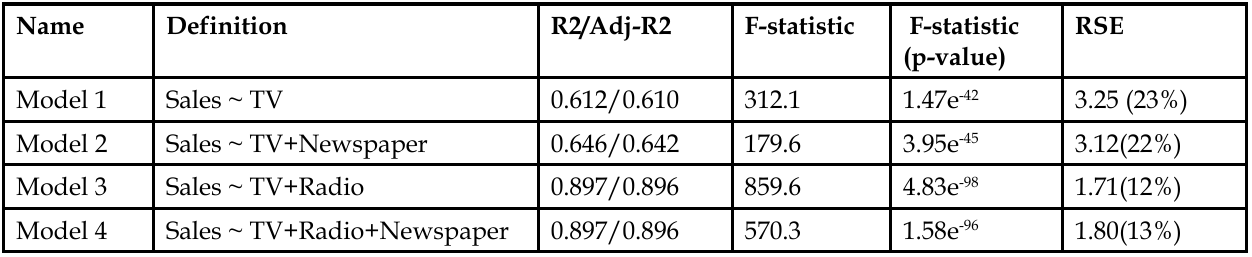
\includegraphics[width=10cm,keepaspectratio=true]{./images/modelsGuide.png}
	\% modelsGuide.png: 0x0 pixel, 300dpi, 0.00x0.00 cm, bb=
	\caption{Variable selection guide.}
	\label{fig:4.10.1}
\end{figure}

Finally, to summarize, for building a reliable linear model, predictor variables should be evaluated and selected according to the following fundamental criteria:
\begin{itemize}
	\item \texttt{$R^2$}: This value will inevitably increase whenever a new predictor variable is added to the model. Therefore, it is not a trustworthy benchmark of whether the model has truly become more efficient. Instead, to verify efficiency, we must examine the adjusted $R^2$. This adjusted metric should increase upon adding a new predictor variable.
	\item \texttt{$p$-value}: The smaller the $p$-value associated with a predictor variable's coefficient estimate, the stronger the empirical justification for including that variable in the model.
	\item \texttt{$F$-statistic}: The value of the overall $F$-statistic for the specification should increase upon including a new predictor variable for that addition to be considered statistically efficient. An upward shift in the $F$-statistic serves as a strong indicator of model improvement attributable specifically to the addition of that variable. Alternatively, the $p$-value associated with the overall $F$-statistic should decrease upon adding the new predictor.
	\item \texttt{RSE}: The Residual Standard Error (`RSE`) for the new model specification should decrease upon adding the new predictor variable.
	\item \texttt{VIF}: To resolve issues arising from multicollinearity, explanatory variables exhibiting excessively high Variance Inflation Factor (`VIF`) values should be pruned from the specification.
\end{itemize}
